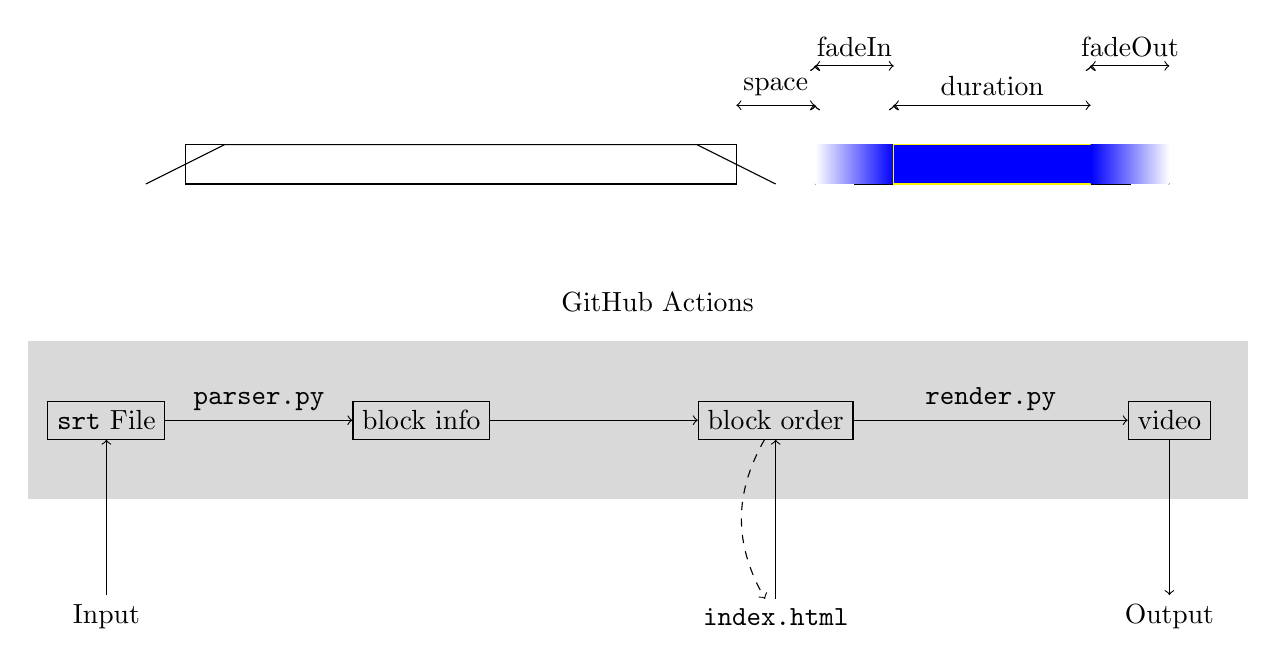
\begin{tikzpicture}
 \tikzstyle{steps} = [draw];
 \tikzstyle{flow} = [->];
 \draw [flow, fill=gray!30, draw=none] (-5,2.5) rectangle (10.5,0.5);
\node [steps] (v1) at (-4,1.5) {\texttt{srt} File};
\node [steps] (v2) at (0,1.5) {block info};

\draw [flow] (v1) edge node [above, font=\ttfamily] {parser.py} (v2);
\node [steps] (v3) at (4.5,1.5) {block order};
\draw  (-3,5) rectangle (4,4.5);
\draw (-3.5,4.5) -- (-2.5,5) -- (3.5,5) -- (4.5,4.5);
\draw  (5.5,5) rectangle (9,4.5);
\draw (5,4.5) -- (6,5) node (v8) {} -- (8.5,5) -- (9.5,4.5);
\draw[<->] (5,5.5) edge node [above] {space} (4,5.5);

\draw[<->] (5,6) edge node [above] {fadeIn} (6,6);
\draw[<->] (6,5.5) edge node[above] {duration} (8.5,5.5);

\draw [<->] (8.5,6) edge node [above] {fadeOut} (9.5,6);
\draw [flow] (v2) edge (v3);
\node [steps] (v4) at (9.5,1.5) {video};
\draw [flow] (v3) edge node [above, font=\ttfamily] {render.py} (v4);
\node [font=\ttfamily] (v5) at (4.5,-1) {index.html};
\draw [flow] (v5) edge (v3);
\node (v6) at (-4,-1) {Input};
\draw [flow] (v6) edge (v1);
\node at (3,3) {GitHub Actions};
\node (v7) at (9.5,-1) {Output};

\draw [flow] (v4) edge (v7);
\draw [flow, dashed] (v3) edge [bend right] (v5);
\draw [left color=white, right color=blue, draw = none]  (5,5) rectangle (6,4.5);
\draw [fill=blue, draw=yellow] (8.5,4.5) rectangle (v8);
\draw [left color=blue, right color=white, draw=none] (9.5,5) rectangle (8.5,4.5);

\end{tikzpicture}